\documentclass[12pt]{article}
\usepackage{amsmath}
\usepackage{amssymb}
\usepackage[letterpaper,margin=0.85in,centering]{geometry}
\usepackage{fancyhdr}
\usepackage{enumerate}
\usepackage{lastpage}
\usepackage{multicol}
\usepackage{graphicx}
\usepackage{tikz}
\usetikzlibrary{calc, positioning, decorations.pathmorphing}


\reversemarginpar

\pagestyle{fancy}
\cfoot{}
\lhead{Math 1560}\chead{Test \# 3 Solutions }\rhead{June 1st, 2017}
%\rfoot{Total: 10 points}
%\chead{{\bf Name:}}
\newcommand{\points}[1]{\marginpar{\hspace{24pt}[#1]}}
\newcommand{\skipline}{\vspace{12pt}}
%\renewcommand{\headrulewidth}{0in}
\headheight 30pt

\newcommand{\di}{\displaystyle}
\newcommand{\abs}[1]{\lvert #1\rvert}
\newcommand{\len}[1]{\lVert #1\rVert}
\renewcommand{\i}{\mathbf{i}}
\renewcommand{\j}{\mathbf{j}}
\renewcommand{\k}{\mathbf{k}}
\newcommand{\R}{\mathbb{R}}
\newcommand{\aaa}{\mathbf{a}}
\newcommand{\bbb}{\mathbf{b}}
\newcommand{\ccc}{\mathbf{c}}
\newcommand{\dotp}{\boldsymbol{\cdot}}
\newcommand{\bbm}{\begin{bmatrix}}
\newcommand{\ebm}{\end{bmatrix}}                   
                  
\begin{document}

%\author{Instructor: Sean Fitzpatrick}
\thispagestyle{fancy}
%\noindent{{\bf Name and student number:}}

 \begin{enumerate}
 \item  Compute the derivatives of the following functions:
\begin{enumerate}
 \item $f(x) = \arctan(x)$ \points{2}

\bigskip

\[
 f'(x) = \frac{1}{1+x^2}
\]

\bigskip

 \item $g(x) = \arcsin(x^3)$ \points{2}

\bigskip

\[
 g'(x) = \frac{1}{\sqrt{1-(x^3)^2}}\frac{d}{dx}(x^3) = \frac{3x^2}{\sqrt{1-x^6}}.
\]

\bigskip

 \item $h(x) = \sec(\arccos(x))$ \points{2} \quad (Hint: simplify first!)

\bigskip

We note that $\sec(\arccos(x)) = \dfrac{1}{\cos(\arccos(x))} = \dfrac{1}{x}$. Therefore,
\[
 h'(x) = \frac{d}{dx}\left(\frac{1}{x}\right) = \frac{d}{dx}(x^{-1}) = -x^{-2} = -\frac{1}{x^2}.
\]

\bigskip


\end{enumerate}

\item Find $\dfrac{dy}{dx}$ in terms of $x$ and $y$ given that \points{3} $\sin(y)=x^2y^3$.

\bigskip

Differentiating both sides of $\sin(y)=x^2y^3$ with respect to $x$, we find
\[
 \cos(y)\frac{dy}{dx} = 2xy^3+3x^2y^2\frac{dy}{dx}.
\]
Solving for $\frac{dy}{dx}$, we find
\[
 \frac{dy}{dx} = \frac{2xy^3}{\cos(y)-3x^2y^2}.
\]

\newpage

\item Consider the function $f(x)=3x^5-5x^3$.
\begin{enumerate}
 \item Compute $f'(x)$ \points{1}

\medskip

\[
 f'(x) = 15x^4-15x^2=15x^2(x^2-1)=15x^2(x-1)(x+1).
\]

\medskip

 \item Construct a sign diagram for $f'(x)$. \points{1}

\medskip

From part (a), the zeros of $f'$ are at $x=-1$, $x=0$, and $x=1$. Our sign diagram is given by
\begin{center}
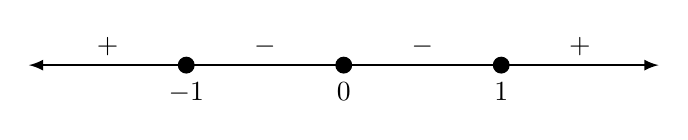
\begin{tikzpicture}[>=latex]
  \draw [thick, <->] (-4,0) -- (4,0);
  \draw [fill] (-2,0) circle [radius =.1];
  \draw [fill] (0,0) circle [radius =.1];
  \draw [fill] (2,0) circle [radius =.1];
  \node at (-3,0) [above] {$+$};
  \node at (-1,0) [above] {$-$};
  \node at (1,0) [above] {$-$};
  \node at (3,0) [above] {$+$};
  \node at (-2,-0.1) [below] {$-1$};
  \node at (0,-0.1) [below] {$0$};
  \node at (2,-0.1) [below] {$1$};
  \end{tikzpicture}
\end{center}

\bigskip

 \item Classify each critical point of $f(x)$ \points{1} as a local minimum, local maximum, or neither.

\bigskip

Using the first derivative test, we see that $f$ has a local maximum at $(-1,f(-1))=(-1,2)$, and a local minimum at $(1,f(1)) = (1,-2)$. The critical point at $x=0$ is neither a maximum nor a minimum.

\bigskip

 \item Determine the intervals where $f(x)$ is\points{2}
\begin{itemize}
 \item Increasing:

\medskip

$f(x)$ is increasing on $(-\infty,-1)\cup (1,\infty)$

\medskip


 \item Decreasing:

\medskip

$f(x)$ is decreasing on $(-1,1)$.

\medskip

\end{itemize}

 \item Compute $f''(x)$.\points{1}

\medskip

\[
 f''(x) = \frac{d}{dx}(15x^4-15x^2)=60x^3-30x=30x(2x^2-1)=30x(\sqrt{2}x-1)(\sqrt{2}x+1).
\]

\medskip

 \item Construct a sign diagram for $f''(x)$. \points{1}

\medskip

From part (e), the zeros of $f''$ are at $x=-1/\sqrt{2}$, $x=0$, and $x=1/\sqrt{2}$. The sign diagram is given by
\begin{center}
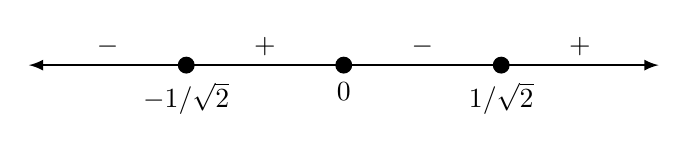
\begin{tikzpicture}[>=latex]
  \draw [thick, <->] (-4,0) -- (4,0);
  \draw [fill] (-2,0) circle [radius =.1];
  \draw [fill] (0,0) circle [radius =.1];
  \draw [fill] (2,0) circle [radius =.1];
  \node at (-3,0) [above] {$-$};
  \node at (-1,0) [above] {$+$};
  \node at (1,0) [above] {$-$};
  \node at (3,0) [above] {$+$};
  \node at (-2,-0.1) [below] {$-1/\sqrt{2}$};
  \node at (0,-0.1) [below] {$0$};
  \node at (2,-0.1) [below] {$1/\sqrt{2}$};
  \end{tikzpicture}
\end{center}

 \item Determine the intervals on which the graph of $f$ is\points{2}
\begin{itemize}
 \item Concave up:

\medskip

$f(x)$ is concave up on $(-1/\sqrt{2},0)\cup (1/\sqrt{2},\infty)$.

\medskip

 \item Concave down:

\medskip

$f(x)$ is concave down on $(-\infty, -1/\sqrt{2})\cup(0,1/\sqrt{2})$.
\end{itemize}

\end{enumerate}

\end{enumerate}





\end{document}